% Template for a Computer Science Tripos Part II project dissertation
\documentclass[12pt,a4paper,twoside,openright]{report}
\usepackage[pdfborder={0 0 0}]{hyperref}    % turns references into hyperlinks
\usepackage[margin=25mm]{geometry}  % adjusts page layout
\usepackage{graphicx}  % allows inclusion of PDF, PNG and JPG images
\usepackage{verbatim}
\usepackage{pdfpages} % allows inclusion of non tex project proposal
\usepackage{docmute}   % only needed to allow inclusion of proposal.tex
\usepackage{varwidth}
\usepackage{tikz}
\usetikzlibrary{shapes,arrows,positioning,chains}
\usepackage{listings}
\lstdefinestyle{tree}{
    literate=
    {├}{{\smash{\raisebox{-1ex}{\rule{1pt}{\baselineskip}}}\raisebox{0.5ex}{\rule{1ex}{1pt}}}}1 
    {─}{{\raisebox{0.5ex}{\rule{1.5ex}{1pt}}}}1 
    {└}{{\smash{\raisebox{0.5ex}{\rule{1pt}{\dimexpr\baselineskip-1.5ex}}}\raisebox{0.5ex}{\rule{1ex}{1pt}}}}1 
    {│}{{\smash{\raisebox{-1ex}{\rule{1pt}{\baselineskip}}}\raisebox{0.5ex}{\rule{1ex}{0pt}}}}1 
  }
\usepackage{CJKutf8}
\raggedbottom                           % try to avoid widows and orphans
\sloppy
\clubpenalty1000%
\widowpenalty1000%

\renewcommand{\baselinestretch}{1.1}    % adjust line spacing to make
                                        % more readable
\begin{document}

\bibliographystyle{plain}


%%%%%%%%%%%%%%%%%%%%%%%%%%%%%%%%%%%%%%%%%%%%%%%%%%%%%%%%%%%%%%%%%%%%%%%%
% Title


\pagestyle{empty}

\rightline{\LARGE \textbf{Oliver Black}}

\addcontentsline{toc}{chapter}{Cover Sheet}

\vspace*{60mm}
\begin{center}
\Huge
\textbf{Software IPv6 Router in Rust} \\[5mm]
Computer Science Tripos -- Part II \\[5mm]
Selwyn College \\[5mm]
\today  % today's date
\end{center}

\newpage
\addcontentsline{toc}{chapter}{Declaration of Originality}
\section*{Declaration of Originality}

I, Oliver Black of Selwyn College, being a candidate for Part II of 
the Computer Science Tripos, hereby declare
that this dissertation and the work described in it are my own work,
unaided except as may be specified below, and that the dissertation
does not contain material that has already been used to any substantial
extent for a comparable purpose.

\bigskip
\leftline{Signed Oliver Black}

\medskip
\leftline{Date \today}

%%%%%%%%%%%%%%%%%%%%%%%%%%%%%%%%%%%%%%%%%%%%%%%%%%%%%%%%%%%%%%%%%%%%%%%%%%%%%%
% Proforma, table of contents and list of figures

\pagestyle{plain}

\chapter*{Proforma}
\addcontentsline{toc}{chapter}{Proforma}

{\large
\begin{tabular}{ll}
Name:               & \bf Oliver Black                      \\
College:            & \bf Selwyn College                     \\
Project Title:      & \bf Software IPv6 Router in Rust \\
Examination:        & \bf Computer Science Tripos -- Part II, July 2001  \\
Word Count:         & \bf 6000 \footnotemark[1]
                       \\
Project Originator: & Oliver Black \& Richard Watts      \\
Supervisor:         & Andrew Moore                   \\ 
\end{tabular}
}
\footnotetext[1]{This word count was computed
by copying the relevant part of the dissertation into \url{https://wordcounter.net/}
}
\stepcounter{footnote}


\section*{Original Aims of the Project}

The IPv6 standard contains a large number of complex requirements, complicating understanding. I aim to design and implement a simple IPv6 router (called Luyou) using Rust\cite{rust} that behaves as specified in the IPv6 RFCs\cite{ipv6_rfc}. This router should implement the minimum functionality required by the relevant standards, yet still be functional, minimal, \& stable.  Rust is a new programming language that aims to be as fast as C while maintaining memory safety, I wanted to understand how practical it was to develop in.

\section*{Work Completed}

Despite having initial difficulties setting up my test environment (called Luxing) using Mininet\cite{mininet}, due to its lack of support for IPv6, I successfully implemented a functioning IPv6 router in rust that met almost all of my core requirements. Both the Luyou itself, and the Luxing, are available for public use.  TODO mention speedup/code coverage/size/RFC coverage/throughput AND fill rest in when main body done. mention how ambitious original claims were

\section*{Special Difficulties}

None. TODO fill in

\tableofcontents
\addcontentsline{toc}{chapter}{Table of Contents}
\listoffigures
\addcontentsline{toc}{chapter}{List of Figures}

\newpage
\section*{Acknowledgements}

Many thanks to:
\begin{itemize}
\item My supervisor Andrew Moore for his helpful advice.
\item My Director of Studies Dr Richard Watts for his guidance.
\item Friends \& family for proofreading.
\end{itemize}

%%%%%%%%%%%%%%%%%%%%%%%%%%%%%%%%%%%%%%%%%%%%%%%%%%%%%%%%%%%%%%%%%%%%%%%
% now for the chapters

\pagestyle{headings}

\chapter{Introduction}
\label{chap::introduction}
Slowly but surely the internet is making progress towards IPv6, but how do pages of Requests for Comments (RFCs) translate into real world network components? The aim of this project was to develop an IPv6 Router in Rust (Luyou) that explores the functionality of IPv6, and how different parts of the various standards fit together. The project has been a success, I have produced a functioning router and accompanying test suite (Luxing).

\bigskip

The router is called Luyou as \begin{CJK}{UTF8}{gbsn}路由器\end{CJK} (Luyouqi) is Chinese for router, and the router was primarily written while travelling in China, and \begin{CJK}{UTF8}{gbsn}旅游\end{CJK} (Luyou) is Chinese for travelling. \begin{CJK}{UTF8}{gbsn}旅行\end{CJK} (Luxing) is also Chinese for travelling, but could also mean \begin{CJK}{UTF8}{gbsn}路行\end{CJK} (Luxing) which could be taken to be an abbreviation for ``Router, OK'', so Luxing is the name of my test bench. The small test client and test server are called Luxingke and Luxingfu respectively, as \begin{CJK}{UTF8}{gbsn}客\end{CJK} (Ke) is client and \begin{CJK}{UTF8}{gbsn}服\end{CJK} (Fu) is server.

\bigskip

Due to the popularity of the Internet, there are now not enough IPv4 addresses to go around. IPv6 is the incoming internet addressing standard that solves numerous issues with IPv4.  Primarily it increases the number of addresses, however it also fixes many flaws in the IPv4 design, and standardises common non-standard practices. For example, the Time To Live in IPv4 was defined partly in terms of seconds left to live\cite{ipv4_rfc}, but in practice was just decremented by 1 on every hop between nodes. In IPv6 the field is accurately renamed to Hop Limit, and is now defined in terms of hops between nodes (as opposed to seconds). Many subtle decisions like this have gone into the IPv6 standard, with an aim to making an internet that works well, rather than one that just works.

\bigskip

Rust\cite{rust} is an up and coming modern low level programming language. It aims to match the performance of C/C++ without sacrificing memory safety, and avoiding garbage collection. It does this through zero-cost high level abstractions such as \textit{ownership} and \textit{lifetimes}. For example, if you pass something to a function, that function then owns that and everything it owns, with it being inaccessible after the function returns. It is possible for functions to borrow values instead, using `\verb!&!', similar to passing by reference.  I chose Rust for my project as it can be easier to debug than C or C++, but mainly because I was interesting in learning Rust.

\bigskip

Mininet\cite{mininet} is an open source virtual network simulator that was developed at Stanford and until 2016 was used in the Part 1B Computer Networking course, it is written in Python.  It creates lightweight virtual networks by making use of Linux's \textit{networked namespaces}, allowing processes to share a kernel, yet be behind different network interfaces. This made it the ideal candidate to build Luyou and Luxing on top of. A simple IPv4 router\cite{simple_router} already exists, and can be ran on top of Mininet, it explores how IPv4 works quite effectively.  Seeing this was one of the key inspirations for my project.

\bigskip

Routers are the backbone of the internet, at the most simple level many of them have a \textit{control plane} that deals with addressing, and a \textit{forwarding plane} that deals with actually sending packets. There are many open source routers out there, but almost all of them have lots of IPv4 code. This makes it difficult to isolate and understand how the IPv6 part actually works.  Starting from scratch allows you to avoid having to deal with IPv4 at all.  

\bigskip

Using the IPv6 standard as a framework, combined with some knowledge about the internals of routers, it is possible to develop and IPv6 router that is stable, small, simple, \& fast.  Such a router could continue to be developed until it could be deployed on actual hardware, but the implementation and testing required meant this was not an objective of this project.  Instead, the aim is to develop a router that implements a sub-set of the IPv6 standard, hopefully including everything an IPv6 router is required by the standards to implement.  In the remainder of this dissertation I will discuss the preparation, implementation, and evaluation of this project.

\chapter{Preparation}
\label{chap::preperation}

Before starting the implementation lots of research and design needed to be done. Lots of research was done into IPv6 RFCs and which aspects were required to be implemented, and which were not. The router software was then designed to provide a framework within which these aspects could be implemented.  Additionally a test plan needed to be made, to enable effective evaluation of the finished product.

\section{Starting Point}
This project was in areas I was interested in and had some experience in. Those areas were all, however, approached from new angles:
\begin{itemize}
\item \textbf{Low-level Systems Programming:} As well as the Part 1B C course I had done several internships that involved a substantial amount of low-level programming in C. However I had never written any project in Rust before.
\item \textbf{Network Programming:} I had completed the Part 1B Computer Networking course, so had some theoretical understanding.  I had also worked on side assignment of a large networking project during an internship.  However I had never worked on a networking project by myself from the ground up before.
\item \textbf{Testing:} I had obviously written tests for my own code before, and had been exposed to large testing frameworks during internships.  However I had never devised my own formal test plan and developed my own test bench before. I also only had brief experience with Python.
\end{itemize}
In terms of existing software, the following where used or built upon by my project:
\begin{itemize}
\item \textbf{pnet}\cite{pnet_rust} the packet and interface libraries in pnet allowed packets to be received, and for individual packets to be manipulated.
\item \textbf{Mininet}\cite{mininet} allowed virtual network environments on Linux to be setup with IPv4 addresses.
\end{itemize}

\section{Research}
An analogous project for IPv4 called Simple Router already exists\cite{simple_router} (it used to be a recommended extension task for the Part 1B Computer Networking course).  It is implemented in C, but it ran on top of Mininet.  The implementation didn't help at all (due to being in C and for IPv4), but it running on Mininet demonstrates that running a router on Mininet is feasible.  Additionally the Mininet python code that ran the Simple Router's executable helped me in designing Luxing.

\bigskip

Most of my research time however was spent reading RFCs related to IPv6.  The main RFC\cite{ipv6_rfc} specifies everything you need to know about IPv6 packets. This describes the contents of the main IPv6 header, \hyperref[fig::ipv6_header]{Figure }\ref{fig::ipv6_header}, including how the fields (e.g. \textit{Hop Limit}) are modified for packets in transit. Additionally this includes the extension headers that need to be implemented by a router, when the packet in question is not addressed to the router this turns out to be none. 

\begin{figure}
\centering
\begin{varwidth}{\linewidth}
\begin{verbatim}
+-+-+-+-+-+-+-+-+-+-+-+-+-+-+-+-+-+-+-+-+-+-+-+-+-+-+-+-+-+-+-+-+
|Version| Traffic Class |           Flow Label                  |
+-+-+-+-+-+-+-+-+-+-+-+-+-+-+-+-+-+-+-+-+-+-+-+-+-+-+-+-+-+-+-+-+
|         Payload Length        |  Next Header  |   Hop Limit   |
+-+-+-+-+-+-+-+-+-+-+-+-+-+-+-+-+-+-+-+-+-+-+-+-+-+-+-+-+-+-+-+-+
|                                                               |
+                                                               +
|                                                               |
+                         Source Address                        +
|                                                               |
+                                                               +
|                                                               |
+-+-+-+-+-+-+-+-+-+-+-+-+-+-+-+-+-+-+-+-+-+-+-+-+-+-+-+-+-+-+-+-+
|                                                               |
+                                                               +
|                                                               |
+                      Destination Address                      +
|                                                               |
+                                                               +
|                                                               |
+-+-+-+-+-+-+-+-+-+-+-+-+-+-+-+-+-+-+-+-+-+-+-+-+-+-+-+-+-+-+-+-+
\end{verbatim}
\end{varwidth}
\caption{IPv6 Header Format\cite{ipv6_rfc}}
\label{fig::ipv6_header}
\end{figure}

\bigskip

Another important RFC was the Internet Control Messaging Protocol RFC\cite{icmpv6_rfc}.  This protocol accompanies IPv6 proper, and must be implemented by all IPv6 routers.  It allows, among other things, errors about dropped packets to be sent back to the source, and \textit{Echo Request/Reply} (ping) messages to be sent.  Alongside this it was important to gain an understanding of how IPv6 related to the link layer below and the transport layer above.

\bigskip

The IPv6 Addressing RFC\cite{ipv6_rfc_adr} contains all you could want to know about the various kinds of IPv6 addresses. However, it is mainly just a list of address ranges and whether they have any special behaviour, it doesn't affect the design of a router much.  I also consulted a few more RFCs related to features that didn't \textit{need} to be implemented by an IPv6 router, more details on those can be found under \hyperref[appendix::requirements]{Appendix A}.

\bigskip

Finally I spent some time researching rust, as it was a new language to me, and I didn't want to make mistakes early on in my implementation that would make things much harder later on.  I discovered a library called pnet\cite{pnet_rust} which implemented low level networking functions and packet abstractions, exactly what I would need.

\section{Analysis}

After finishing my research I needed to do some \textit{requirements analysis} to workout what exactly Luyou (my router) needed to implement, and in what order I should go about implementing them.  I divided up the requirements as recommended into \textit{core} and \textit{extension}, where core contained everything an IPv6 router \textit{needed} to do (according to the RFCs), and extension things I thought I would like it to do as well.  Core was further divided up into \textit{basic} and \textit{advanced}, with basic being everything a router required to provide some form of basic testable functionality, and extension being everything else that was \textit{needed}.

\bigskip

There are three main areas of requirements:
\begin{itemize}
\item Addressing
\item Packet inspection \& forwarding
\item Error reporting \& ICMPv6\cite{icmpv6_rfc}
\end{itemize}

\bigskip

The requirements for addressing can be divided into two parts, the address discovery mechanism (static, SLAAC\cite{slaac_rfc} or DHCPv6\cite{dhcpv6_rfc}) and different address types (Unicast, Anycast, Multicast).  

Although DHCPv6 and SLAAC are both practical and interesting, they aren't \textit{needed} for an RFC router - static addressing is sufficient - so they were put as extension requirements.  Static addressing means the relationship between IPv6 addresses and link layer interfaces is defined when the router starts based on a fixed configuration. In order to get the router forwarding packets as quickly as possible an additional requirement of \textit{flooding} addressing was added.  This is not defined in the RFC for IPv6, as it means a router would instead by functioning as a link layer switch, sending all incoming packets out on all interfaces. Static addressing was \textit{needed} by the RFCs and I decided flooding alone wouldn't really constitute basic testable functionality (of a router). So static addressing is a basic core requirement, with DHCPv6 and SLAAC being extension requirements.

Address types in IPv6 are well defined by the addressing RFC\cite{ipv6_rfc_adr}, hand a router \textit{needs} to deal with all of them.  However, in order to test basic functionality only Unicast really needs to be implemented, as Anycast and Multicast are just mappings from a 'Unicast' address to many Unicast addresses. So Unicast is a basic core requirement, with Anycast and Multicast being advanced core requirements. IPv6 also includes scope for local only addresses, as well as a variety of other specific types, these could also have been extension requirements.

\bigskip

Every packet a router receives needs to be sent to the right destination, and any packet for which the destination is unknown should be sent to the default route. This falls under static addressing as my requirements don't differentiate between the control and data plane - see \hyperref[sec::design]{Design}.  However the payload length must be checked to see if it matches the actual length of the payload - and the packet discarded if not.  Additionally the hop limit must be checked, if it is 1 or 0 the packet should be discarded, otherwise it should be decreased by 1.  Both of these are basic core requirements, they are \textit{needed} and without them it is hard to test basic functionality. Without hop-limit decrements a router leaves packets unaffected, so it is hard to tell if they went through a router at all.

IPv6 also has many extension headers, but they \textit{need} to be ignored by intermediate nodes (for example, fragmentation can only be done by the source and destination nodes), except for the \textit{hop-by-hop options header} which can be ignored by intermediate nodes. Apart from ICMPv6 packets Luyou does not deal with packets that are encapsulated by IPv6 packets (including transport layer protocols).  This means that it does not need to process any headers at all, except for ICMPv6 packets.

\bigskip

ICMPv6 works alongside IPv6 to send informational and error messages between nodes.  These messages include destination, packet size, hop limit, \& header error messages, and echo request \& reply informational messages. One slightly odd requirement relates back to hop-limit in the IPv6 header, if an arriving packet has a hop limit of 1, it should be discarded, unless the destination node is the router in question.  This only occurs for ICMPv6 messages with Luyou, as it does not support receiving any other packets

ICMPv6 is \textit{needed} for any IPv6 router.  However, in order to test the basic functionality of Luyou it was not required. This is because error reporting functions can be, in part, replaced by log output from Luyou itself. As such, ICMPv6 is an advanced core requirement.

\bigskip

Additionally I thought about what my project did not need to do. I have already discussed briefly in my \hyperref[chap::introduction]{Introduction} that I did not want to require Luyou to necessarily be able to be ran on actual hardware, as this would add needless complexity when my aim is to explore and illuminate the IPv6 requirements. 

I did not want to bother with any experimental/unused features, as they don't much help understand the IPv6 requirements. For example the flow label in the IPv6 header can in theory be used to prioritise real time packets, and several other uses have been suggested, however it can just be ignored by the standard, and I believe that is what many routers do.  The same can be applied to many IPv6 extension headers, I planned to evaluate all my extension requirements to see if they met this criterion after finishing my core requirements.

I didn't want to get involved with cross-layer optimisations, as these would also not help to understand the IPv6 requirements.  Secondly, this would not be particularly useful, as the nature of Mininet creating perfect virtual ethernet links means Luyou has few bottlenecks, but it is often in bottlenecks that such cross-layer optimisations are used.

Mininet does allow for artificially reducing the MTU of links, and through the help of helper applications artificially dropping packets and increasing latency.  However, my aim was not to produce a high performance router, so any requirement based on performance was also not what I was looking for.

\bigskip

To summarise, here are the requirements for Luyou, categorised by type, starting with my basic core requirements:
\begin{itemize}
\item Send packets to the correct hardware interface in accordance with the static routing rules provided
\item Deal with IPv6 headers in accordance with the standard (Hop limit, etc)
\end{itemize}
My advanced core requirements:
\begin{itemize}
\item ICMPv6
\item Multicast
\item Anycast
\end{itemize}
My extension requirements:
\begin{itemize}
\item IPv6 extension headers
\item DHCPv6
\item SLAAC
\end{itemize}
My non-goals, things that would needlessly complicate the project:
\begin{itemize}
\item To be stable, complete, fast, \& compatible enough to be easily run on real hardware in a real world environment.
\item Implementing experimental or unused features - specifically those potentially covered by my extension requirements.
\item Higher layer packet inspection
\item Performance based goals (throughput, etc)
\end{itemize}
For a formal list of the requirements I came up with (along with identifiers and associated tests) see \hyperref[appendix::requirements]{Appendix A}.

\section{Design}
\label{sec::design}

Having completed my analysis and produced a structured list of requirements the next step was to come up with a design for Luyou that would enable me to implement these requirements.  There were two main ideas in the design Luyou itself itself (the design of the Luxing (the test bench) is discussed in the next section). 

\bigskip

The first was the separation of the control and forwarding plane, which by itself is nothing special, but the design in software was slight more complex.  As always, the control plane deals with the addressing (along with other aspects and the forwarding plane with link layer interfaces and individual packets.  The two communicate through forwarding tables (in the case of non static addressing communication in the other direction is also required). The forwarding plane in my case is made up of a pair of threads for each interface, one receiving and one transmitting. All of the receiving threads have read access to two objects, one is the routing table produced by the control plane, the other is a map of hardware addresses to channels.  The channel each hardware address is linked to leads to the transmitting thread for the interface of that hardware address (See \hyperref[fig::router_design]{Figure }\ref{fig::router_design}). Read \hyperref[chap::implementation]{Implementation} for specifics.

\begin{figure}
\centering
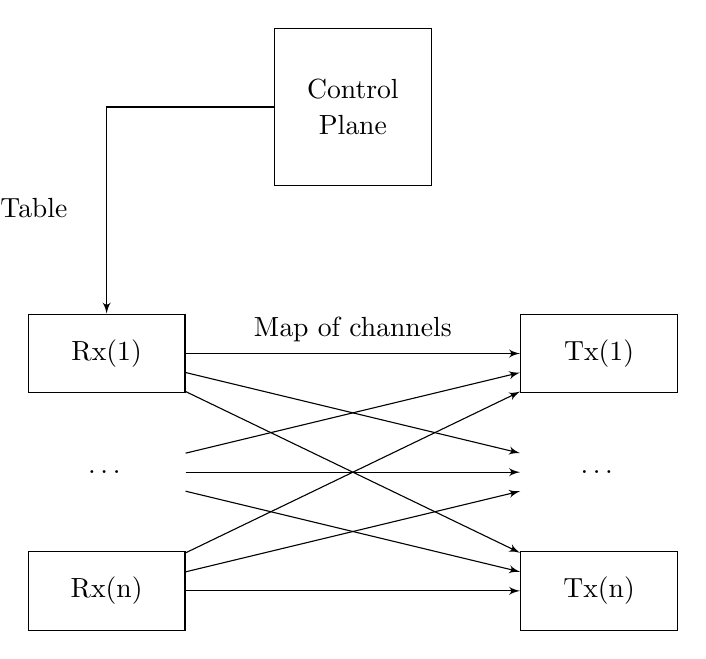
\begin{tikzpicture}
\tikzstyle{block} = [rectangle, draw, 
    text width=5em, text centered, minimum height=2cm,node distance = 2cm]
\tikzstyle{middle} = [text width=5em, text centered, minimum height=1cm,node distance = 2cm]
\tikzstyle{little} = [rectangle, draw, middle]
\tikzstyle{line} = [draw, -latex']

\node [block] (control) {Control Plane};
\node [below=of control, yshift=-10mm] (center) {};
\node [little, left=of center] (recv1) {Rx(1)};
\node [little, below=of recv1] (recv2) {Rx(n)};
\node [little, right=of center] (trans1) {Tx(1)};
\node [little, below=of trans1] (trans2) {Tx(n)};

\path (recv1) -- node [middle] (midl){\ldots} (recv2);

\path (trans1) -- node [middle] (midr){\ldots} (trans2);

\path [line] (control) -|
node [near end, transform canvas={xshift=-16mm}] {Routing Table}
(recv1);

\path  [line] (recv1) -- node [transform canvas={yshift=+3mm}] {Map of channels} (trans1);
\path  [line] (recv1) -- (trans2);
\path  [line] (recv1) -- (midr);

\path  [line] (midl) -- (trans1);
\path  [line] (midl) -- (trans2);
\path  [line] (midl) -- (midr);

\path  [line] (recv2) -- (trans1);
\path  [line] (recv2) -- (trans2);
\path  [line] (recv2) -- (midr);

\end{tikzpicture}
\caption{Router Design}
\label{fig::router_design}
\end{figure}

\bigskip

The second was designing the layer separation inherent in the TCP/IP stack into Luyou.  This was achieved by having a different function handle each layer, and only passing necessary information between the functions.  There are three layers, Ethernet, IPv6, and ICMPv6 in Luyou, so there are three functions, with only the packets themselves and the relevant addresses being passed between the functions. The Ethernet function sends the IPv6 packet to the IPv6 function, which returns the new IPv6 packet, and the hardware address to send it to.  The IPv6 function sends the ICMPv6 packet along with the source and destination address to the ICMPv6 function, which returns the new ICMPv6 packet along with the new source and destination addresses (See \hyperref[fig::layer_separation]{Figure }\ref{fig::layer_separation}).

\begin{figure}
\centering
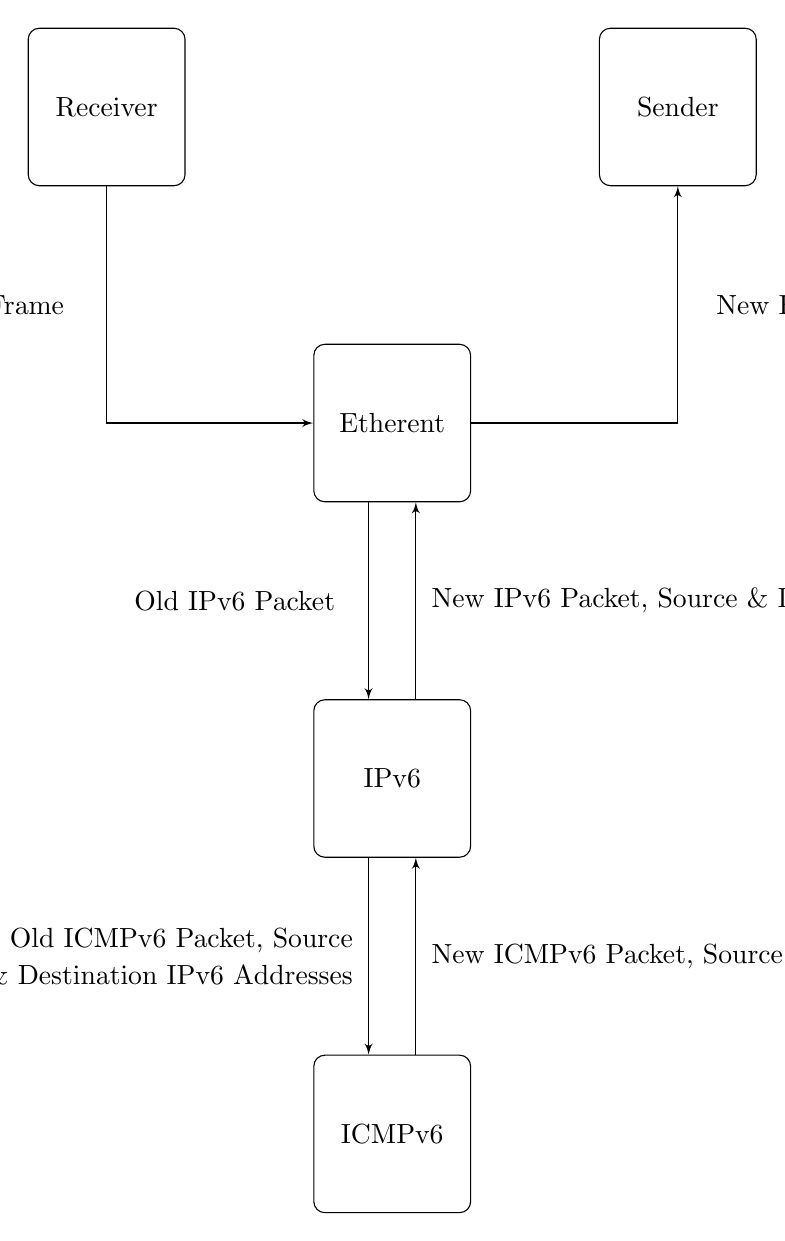
\begin{tikzpicture}

\tikzstyle{block} = [rectangle, draw, 
    text width=5em, text centered, rounded corners, minimum height=2cm,node distance = 2.5cm]
\tikzstyle{invisible} = [rectangle,minimum height=1cm]
\tikzstyle{line} = [draw, -latex']

\node [invisible] (anchor) {};
\node [block, left=of anchor] (receiver) {Receiver};
\node [block, right=of anchor] (sender) {Sender};
\node [block, below=of anchor] (ethernet) {Etherent};
\node [block, below=of ethernet] (ipv6) {IPv6};
\node [block, below=of ipv6] (icmpv6) {ICMPv6};

\path [line] (receiver) |- 
node [near start, transform canvas={xshift=-21mm}] {Old Ethernet Frame} 
(ethernet);
\path [line] (ethernet) -| 
node [near end, transform canvas={xshift=+21mm}] {New Ethernet Frame} 
(sender);
\path [line] (ethernet) edge [transform canvas={xshift=-3mm}] 
node [transform canvas={xshift=-17mm}] {Old IPv6 Packet}
(ipv6);
\path [line] (ipv6) edge [transform canvas={xshift=+3mm}] 
node [transform canvas={xshift=+42mm}, text width=8cm, align=left] {New IPv6 Packet, Source \& Destination MACs}
(ethernet);
\path [line] (ipv6) edge [transform canvas={xshift=-3mm}] 
node [transform canvas={xshift=-42mm}, text width=8cm, align=right] {Old ICMPv6 Packet, Source \& Destination IPv6 Addresses}
(icmpv6);
\path [line] (icmpv6) edge [transform canvas={xshift=+3mm}] 
node [transform canvas={xshift=+42mm}, text width=8cm, align=left] {New ICMPv6 Packet, Source \& Destination MACs}
(ipv6);
\end{tikzpicture}
\caption{Layer Separation}
\label{fig::layer_separation}
\end{figure}

\bigskip

Both of these design choices made the implementation much easier, separating the code into functionally separate sections, reducing the risk of introducing bugs, and most importantly providing a structured framework within which to code.

\section{Test Plan}
\label{sec:test_plan}

With requirements and a design of Luyou completed, I needed to come up with a plan of how I was going to verify that Luyou was functioning as expected.  This was divided into two parts, the design of Luxing, and secondly the list of tests to be run on it.

\bigskip

I planned to make Luxing from Mininet and a couple of helper applications (either written in Python or Rust).  Some helper applications would be capable of sending packets with specific properties, and outputting any packets they received. Other helper applications would do more complicated end to end testing, such as running a web server and requesting web pages.  Unfortunately I found Mininet's IPv6 support was far less complete than I had believed in my \hyperref[project_proposal]{Project Proposal}.  I either had to write my own network emulation environment from scratch, or develop some kind of modification or wrapper for Mininet.  I chose to focus on a wrapper that would intercept the functions I needed to use, and change the necessary things to get Mininet working, details of this wrapper can be found in \hyperref[chap::implementation]{Implementation}.

\bigskip

When formalising the results of my analysis into a list of tests there were two key steps. The first, a one, was numbering everything so I wouldn't get lost or forget any requirements.  Secondly I had to come up with the tests themselves, this normally included a test for the given functionality when it should happen, a test for it not happening when it shouldn't happen, and any edge case tests I could thing of.  For example, hop limit decrement, when a packet passes through a router its hop limit should be decreased by 1 and the packet sent on its way; when the packet has a hop limit of 1 or 0 on arrival it should be dropped and not sent on its way, and if, the packet has a hop limit of 1 and is addressed to the router it should not be dropped, it should instead be handed up a layer. 

\bigskip

To avoid all the tests being dependent on an almost complete implementation of Luyou I avoided tests for features relying on other features. If we return to the example hop limit given above Luyou should send an ICMPv6 \textit{Time Exceeded} message when a packet is dropped.  However, this would mean any test for hop limit depends on a correct implementation of ICMPv6, as well as the correct implementation of Hop Limit.  As a result every test can only rely on functionality already implemented.  My numbering system happened to match my planned order of implementation, so just reading off all the previous tests lets you know which features that test potentially relies on.  Back to the hop limit example, this means that success of the hop limit test was judged by the packet not continuing and log messages being outputted by Luyou. When it came to test Time Exceeded though it could rely on the already implemented hop limit, so the planned test involved sending a packet with hop limit 0 and testing for a Time Exceeded response.

\section{Professional Practice}
This is a brief section on preparation related to professional skills and practice.  Two large aspects are testing and software engineering, both of which are explained in detail in the rest of \hyperref[chap::preparation]{Preparation} and in \hyperref[chap::implementation]{Implementation}.  

\bigskip

There could be security exploits in my code, and if anybody would like to adapt my code for use in a real world router I would recommend it is tested extensively.

\bigskip

In terms of licensing my code makes use of Mininet, Rust, the Rust standard library, and pnet.  However, none of these are distributed with my project, so there are no licensing requirements.  That said, my code is released under the GNU GPL\cite{gpl}, which is compatible with their Apache 2.0/MIT licenses.

\bigskip

I don't believe there are any ethical issues involved in my project, and there is no human testing.

\chapter{Implementation}
\label{chap::implementation}

Implementing Luyou was an exciting iterative process, with many challenges, but also a real sense of achievement every time I implemented something I had never done before and again when it passed my tests.  There were two main parts to implement, Luyou (the router itself) and Luxing (the test bench).  Both had their own different challenges.  The relationship between the two is explained in more detail in the third section about \hyperref[sec::soft_eng] {Software Engineering} practices used.


\addcontentsline{toc}{section}{Repository Overview}
\section*{Repository Overview}

Here is the repository overview, the project is made up of a python application (the test bench - Luxing) and three rust applications (a test client - Luxingke, a test server - Luxingfu, and the router itself - Luyou). To shorten and explain the tree \verb!*comments*! have been added inline. All of these files were written from scratch except for the few examples commented as \verb!from documentation!.

\begin{lstlisting}[style=tree]
.
├── dissertation
│   └── *latex files*
├── python
│   ├── luxing
│   │   ├── __init__.py
│   │   ├── test_*test number*.py
│   │   ├── test_example.py
│   │   ├── test_framework.py *mininet wrapper*
│   │   ├── test_playground.py 
│   │   └── test_tw_example.py *example mininet application from
│   │                           documentation*
│   └── __init__.py
├── rust
│   ├── luxingfu
│   │   └── src
│   │       └── main.rs *test server*
│   ├── luxingke
│   │   └── src
│   │       └── main.rs *test client*
│   └── luyou
│       ├── resource
│       │   └── routing.txt *static routing file*
│       └── src
│           ├── examples
│           │   └── *related examples from documentation*
│           ├── control.rs *control plane*
│           ├── forwarding.rs *forwarding plane*
│           └── main.rs *main router file*
├── COPYING.txt
├── LICENSE.txt
├── README.md
└── test.sh *script to start tests*
\end{lstlisting}


\section{Router}
\label{sec::router}

Luyou was implemented requirement by requirement, as set out in \hyperref[chap::preparation]{Preparation} and\hyperref[appendix::requirements]{Appendix A}.  Version control was performed using git, with backups committed to an \textit{exploratory} branch, with merges into the \textit{master} branch whenever a specific requirement had been completely implemented.

\bigskip

The first thing I did was write a very simple Ethernet repeater, that connected to two interfaces and forwarded all packets as is, on the other interface.  This demonstrated pnet\cite{pnet_rust} worked as I expected, and allowed me to move on, and satisfied the flooding requirement.  The next step was implementing the the shared map of addresses to interfaces to allow forwarding on a specific interface, then a shared routing table to allow working out which interface to forward on, and the separation of layers to allow easily adding IPv6 feautres and ICMPv6 later.

\bigskip

One of the early issues I encountered was implementing a shared map of transmission channels, as described in \hyperref[sec::design]{Design}. There is a method in pnet\cite{pnet_rust} called \verb!channel() -> Channel!, where a \verb!Channel! is a pair of pipes, one receiving and one transmitting.  I planned to give each receiving thread a receiving pipe, and give them all a map from MAC address to transmitting pipe for the sending address.  Unfortunately the pipe type used by pnet does not support sharing across threads (and this is enforced by the rust type system). So instead I had to have one additional thread for each transmitting pipe, with another thread safe pipe receiver associated with each transmitting thread, and all the corresponding transmitting thread safe pipes in the map.  This worked without much issues, partly because the map never changed, so was cloned across threads.  See \hyperref[fig::sending]{Figure }\ref{fig::sending} for the code that creates a thread safe channel. Also, the packet representations used by pnet can't be sent over a channel used by multiple threads, as they don't implement the \verb!Clone! trait, however the underlying byte buffer does implement the \verb!Clone! trait. A trait in Rust is similar to an interface in a language like Java.

\begin{figure}
\centering
\begin{varwidth}{\linewidth}
\begin{verbatim}
//SENDER
pub fn start_sender(tx : Box<DataLinkSender>) 
 		-> (JoinHandle<()>, Sender<Box<[u8]>>) {
    let (sender, receiver) = channel();
    let handle = thread::spawn(move || sender_loop(tx, receiver));
    (handle, (sender))
}

fn sender_loop(mut sender: Box<DataLinkSender>, 
			   receiver: Receiver<Box<[u8]>>) {
    loop {
        let packet = receiver.recv().unwrap();
        sender.send_to(&packet,None);
    }
}
\end{verbatim}
\end{varwidth}
\caption{Code for starting a transmitting thread, returning a thread safe pipe}
\label{fig::sending}
\end{figure}

\bigskip

Sharing the routing table between layers was difficult.  I could have just generated a map of IPv6 addresses to MAC addresses on start and shared it analogously to the map of MAC addresses to interfaces. However, my extension goals included implementing DHCPv6 and SLAAC, both of which require the routing table to be editable.  To allow this change without having to edit the forwarding layer too much it made sense to have a separate control thread with write access to the routing table, and give all the reading threads read access.  I did this even though as it stands the control thread sets up the static routing then exits.  Rust enforces safety, so in order to share the structure between threads it needed to be put inside an \verb!Arc! (Atomically Reference Counted)\cite{rust_arc} a thread-safer reference counting pointer.  This doesn't actually support the multiple reader single writer semantics required for DHCPv6 or SLAAC, but simply swapping it out for a RwLock\cite{rust_rwlock} would be sufficient.

\bigskip

The static routing rules themselves were read from a text file (that was created by Luxing). It had quite a simple format, the first line was the IPv6 address of the default route, the second line that of Luyou.  Every following line was an IPv6 address, then by an `\verb!@!' followed by the pair of MAC addresses for the associated interface (separated by a `\verb!,!').  Little validation was performed when parsing this file, as any time spent improving error reporting in the case of invalid files could be better spent working towards implementing DHCPv6 or SLAAC, and rendering the static addressing obsolete. Rust makes reading text files easy, through parsing traits.

\bigskip

Separating each layer was quite simple, the ethernet layer received a packet, called the IPv6 function, which in turn sometimes called the ICMPv6 layer.  My plan was to hand a pair of packets up the layers (the received packet and the new packet to be sent), with each layer stripping off the headers and only handing the rest down to the next layer.  Unfortunately this was complicated by the design of pnet.  A packet in pnet is merely a wrapper for an underlying byte buffer, this is sensible as it reduces copying.  Everything in Rust can only have a maximum of one mutable reference at a time.  A mutable ethernet packet in pnet refers to the entire of the underlying buffer, both header and payload.  This means that if you have a mutable ethernet packet it is impossible to create a mutable IPv6 packet from the payload and then edit both of them.  I believe this is a design flaw in pnet, as the solution is to create a fresh buffer for the ipv6 packet and then copy the payload across, resulting in extra copies. Instead creating a packet from a buffer should return a tuple of the header and the payload, allowing them to be owned and mutated separately, with each owning a different \verb!slice! of the underlying buffer. This can be better seen in  \hyperref[fig::mutability]{Figure }\ref{fig::mutability}.

\begin{figure}
\centering
\begin{varwidth}{\linewidth}
\begin{verbatim}
let mut buffer = vec![0;new_packet.payload().len()];
let mut new_ipv6_packet = MutableIpv6Packet::new(&mut buffer).unwrap();
new_ipv6_packet.set_payload_length(
    (new_packet.payload().len()-40) as u16);

let (source, destination) = 
    match transform_ipv6_packet(
        old_ipv6_packet, &mut new_ipv6_packet, routing) {
    Ok(p) => p,
    Err(e) => return Err(e),
};

new_packet.set_destination(destination);
new_packet.set_source(source);
new_packet.set_ethertype(Ipv6);
new_packet.set_payload(new_ipv6_packet.packet());
\end{verbatim}
\end{varwidth}
\caption{Excerpt from Ethernet layer: creates and IPv6 packet from a new buffer, lends it to the IPv6 layer, then copies the result into the Ethernet packet}
\label{fig::mutability}
\end{figure}

\bigskip

ICMPv6 often requires packets be sent not to their destination, but back to their source address.  Initially this appeared to be a challenge, as it looked like I needed a completely separate path for ICMPv6 packets addressed to Luyou. However due to how I separated the layers this was not necessary. Instead the IPv6 layer passed the old ICMPv6 packet and the old source and destination addresses to the ICMPv6 layer. The ICMPv6 layer then responded with the new ICMPv6 packet, and the new source and destination addresses (for example, with an \verb!Echo Request! ICMPv6 packet, source and destination would be swapped for the \verb!Echo Reply! response).  As long as the IPv6 packet honestly copied these into the new IPv6 packet, and worked out the MAC addresses to pass back to the Ethernet based on the new source and destination addresses, it would work perfectly. This demonstrates how the separation of layers allows new features to leverage existing well tested code effectively, reducing code duplication and increasing reliability.

\section{Test Bench}

As outlined in \hyperref[chap::preparation]{Preparation} a key part of this project is Luxing. Without Luxing it is impossible to verify that Luyou works as expected.  Below I go into detail about how I implemented Luxin, and issues I had.  Solving these issues involved a lot of trial and error, and I didn't have much experience with networking on Linux.

\bigskip

Initially I thought Mininet\cite{mininet} supported IPv6.  However when I set up a network, and tried to use \verb!ping6! between two nodes it didn't work.  This is because Mininet does not support IPv6, and doesn't allocate IPv6 addresses to network nodes.  As described in \hyperref[sec::test_plan]{Test Plan} I chose to write a wrapper for Mininet that added the IPv6 functionality I required.  This wrapper is not as resilient as Mininet itself, it requires operations to be performed in a certain order, that said, it does work, and effectively wraps around Mininet to support IPv6 in a subset of Mininet's use cases.

\bigskip

The first issue I faced was allocating IPv6 addresses to nodes. This was achieved by calling \verb!ifconfig [interface-name] inet6 add [address]! every time a node was added. I then stored the node name and IPv6 address in a two way map, to allow me to easily use the addresses later. My wrapper does not support auto allocating IPv6 addresses, you need to specify an address when you create a node, unlike Mininet which allows IPv4 nodes to be created without an address being specified.

\bigskip

The next big issue came when linking the network up. In general it worked fine, as Mininet links nodes together with Veth (Virtual Ethernet) links, which operate at the link layer.  However, in order to make it easy to debug I wanted to be able to choose mac addresses for each node. As for IPv6 addresses I just had them specified on node creation.  However this didn't work for the router as it had multiple interfaces, so required multiple mac addresses. This was resolved by requiring a MAC address for all links but the first involving the router.

\bigskip

Another issue was adding the default route to all nodes.  In order for ping to work effectively the default route needed to be set to the router for all nodes.  This is easily achievable using the \verb!ip -6 route add default via [default-address] src [node-address]! command, but this didn't work.  This is because when allocated in linux IPv6 addresses take a while before shifting to the \verb!UP! state.  Once I had discovered this I added a loop that slept for 100 milliseconds while the output of \verb!ip -6 addr! contained ``\verb!TENTATIVE!'' before trying to update the default route, this fixed the issue.

\bigskip

As I was using static routing Luxing needed to generate a routing file for the router describing the network it was in.  This was relatively simple, on router start a text file is created, and filled in according to the format described in \hyperref[sec::router]{Router}.  In order to gather the required information whenever a link was added the relevant IPv6 address and source and destination MAC addresses were stored in a map.  Luyou's and the default gateway's addresses also need to be included in the routing file, which required they not be added as ordinary nodes, and instead be added as their own method. For a long time I couldn't get \verb!ping6! to work via my router, through debugging I discovered this was due to \verb!ping6! making use of \textit{Solicited Multicast Addresses} to send requests and responses. A \textit{Solicited Node Multicast} address is most recognisably used by the \cite{Neighbour Discovery Protocol}\cite{ndp_rfc}. Luxing resolves this by adding the addresses to the static routing file, generating them from the already allocated IPv6 addresses.

\bigskip

I also wrote a small test client and server in Rust (called Luxingke and Luxingfu).  Both take an argument that determines which test is being run, the client then produces packets and optionally waits for responses, with the server waiting for packets and optionally producing responses.  By using Rust rather than Python for this I could use pnet, which I understood relatively well by this point, avoiding having to learn a new low level networking library.

\section{Software Engineering}
\label{sec::soft_eng}

Due to both the nature of my project - having to produce a functioning router - and my own personal goals - wanting to learn useful real world skills - I was extremely aware of how I was applying software engineering techniques throughout.

\bigskip

Overall I began by creating a complete list of requirements, then a complete design, then I implemented my router, and then finally I ran all my tests on it.  This is very similar to the \textit{Waterfall} methodology.  This was appropriate (compared to more flexible software engineering methodologies) as my requirements were well defined by RFCs - I did not need to explore and refine requirements as my development progressed. 

\bigskip

However, I didn't really follow the Waterfall methodology as it was not particularly appropriate or sensible to complete my implementation as one large chunk.  Instead I completed several prototypes, each implementing a larger set of the requirements:
\begin{itemize}
\item \textbf{Flooding:} Packets forwarded on all interfaces.
\item \textbf{Static Routing:} Packets forwarded on specific interfaces.
\item \textbf{IPv6 validation:} Invalid IPv6 packets dropped and logged.
\item \textbf{ICMPv6:} Invalid IPv6 packets responded to and echo request/reply implemented.
\end{itemize}
For each of these stages I first refined the requirements (partly based on the success of the last stage), and at the end I would produce a more complete prototype, this is similar to the \textit{Spiral} software development methodology. Doing all of the implementation in one would have prevented me from effectively testing parts of the router independently from each other, and made the final testing much more complex.

\bigskip

Every time I implemented an individual requirement I would write tests for that requirement and run them (ensuring they pass) before proceeding.  Once they passed I would merge my work (on the \textit{exploratory} branch) into the \textit{master} branch, before continuing with the next requirement back on the \textit{exploratory} branch.  Before merging I would also ensure all previous tests passed.  This would involve either fixing Luyou, or in some cases modifying the test itself (for example if it relied on log output that was no longer there due to the implementation of the ICMPv6 response).  By merging often and ensuring my router continued passing all testsjhfdasiuhfdusaiohfdusioaoh

Maye:
Instead I implemented requirements in turn, taking the requirement, further clarifying and refining it (e.g. still processing ICMPv6 packets destined for the router when their hop limit = 1).  I then implemented the requirement, and proceeded to add and run tests before moving on to the next requirement.



\chapter{Evaluation}

WHAT IS HERE AND WHAT IS CONCLUSION

flooding, requirement satisfaction


No requirements for headers, 

Packet in packet out rate limiting
ICMPv6 destination unreachable cannot occur

Extension headers and ICMPv6
ICMPv6 erroneous header, fragment reconstruction, destination unreachable
Local and subnet addresses - maybe explain more earlier
lack of end to end testing
code coverage
difficulties with mininet

Code size 736 lines
How much of RFC (ex references) - IPv6:; Addr: ; ICMPv6: 14 of 18  - unsure
Test coverage - 95%

Routing head not supported - extension headers for ICMPv6 packets
Hop limit doesn’t work with ping

evaluate test bench


\chapter{Conclusion}

Capitilisation, grammar, spelling, test bench or suite, forwarding or data plane, capital Rust, lower case pnet, ethernet caps?
https://www.cl.cam.ac.uk/teaching/projects/pinkbook/node18.html
Search for identifying information
Capitalise MAC
Document of notes and pdf from how to write a dissertation


HOW TO BUILD AND RUN

literature review

add personal goals?

TODO remove TODO

%%%%%%%%%%%%%%%%%%%%%%%%%%%%%%%%%%%%%%%%%%%%%%%%%%%%%%%%%%%%%%%%%%%%%
% the bibliography
\begin{thebibliography}{1}
\addcontentsline{toc}{chapter}{Bibliography}

\bibitem{repo} Software IPv6 Router in Rust repository, the code that accompanies this dissertation, \url{https://github.com/ollie299792458/dissertation-rust-ipv6-router}

\bibitem{rust} Rust, a modern low level programming language, \url{https://www.rust-lang.org/}

\bibitem{mininet} Mininet, a network virtualisation library in Python, \url{http://mininet.org/}

\bibitem{pnet_rust} pnet, a low-level networking API for rust, \url{https://docs.rs/pnet}

\bibitem{rust_arc} Arc, a thread safe reference counted pointer for Rust, \url{https://doc.rust-lang.org/std/sync/struct.Arc.html}

\bibitem{rust_rwlock}RwLock, a multiple reader single writer lock for Rust, \url{https://doc.rust-lang.org/std/sync/struct.RwLock.html}

\bibitem{ipv6_rfc} Internet Protocol, Version 6 (IPv6) Specification, \href{https://tools.ietf.org/html/rfc8200}{RFC 8200}, July 2017

\bibitem{ipv6_rfc_adr} IP Version 6 Addressing Architecture, \href{https://tools.ietf.org/html/rfc4291}{RFC 4291}, February 2006

\bibitem{ipv4_rfc} INTERNET PROTOCOL DARPA INTERNET PROGRAM PROTOCOL SPECIFICATION, \href{https://tools.ietf.org/html/rfc791}{RFC 791}, September 1981

\bibitem{icmpv6_rfc} Internet Control Message Protocol (ICMPv6) for the Internet Protocol Version 6 (IPv6) Specification, \href{https://tools.ietf.org/html/rfc4443}{RFC 4443}, March 2006

\bibitem{slaac_rfc} IPv6 Stateless Address Autoconfiguration, \href{https://tools.ietf.org/html/rfc4862}{RFC 4862}, September 2007

\bibitem{dhcpv6_rfc} Dynamic Host Configuration Protocol for IPv6 (DHCPv6), \href{https://tools.ietf.org/html/rfc3315}{RFC 3315}, July 2003

\bibitem{ndp_rfc} Neighbour Discovery Protocol, Neighbor Discovery for IP version 6 (IPv6), \href{https://tools.ietf.org/html/rfc4861}{RFC 4861}, September 2007

\bibitem{simple_router} Simple Router, implementing an IPv4 router in C on Mininet, \url{https://github.com/mininet/mininet/wiki/Simple-Router}

\bibitem{gpl} GNU General Purpose License, \url{https://www.gnu.org/licenses/quick-guide-gplv3.html}

\end{thebibliography}

%%%%%%%%%%%%%%%%%%%%%%%%%%%%%%%%%%%%%%%%%%%%%%%%%%%%%%%%%%%%%%%%%%%%%
% the appendices
\appendix

\chapter{Requirements}
\label{appendix::requirements}
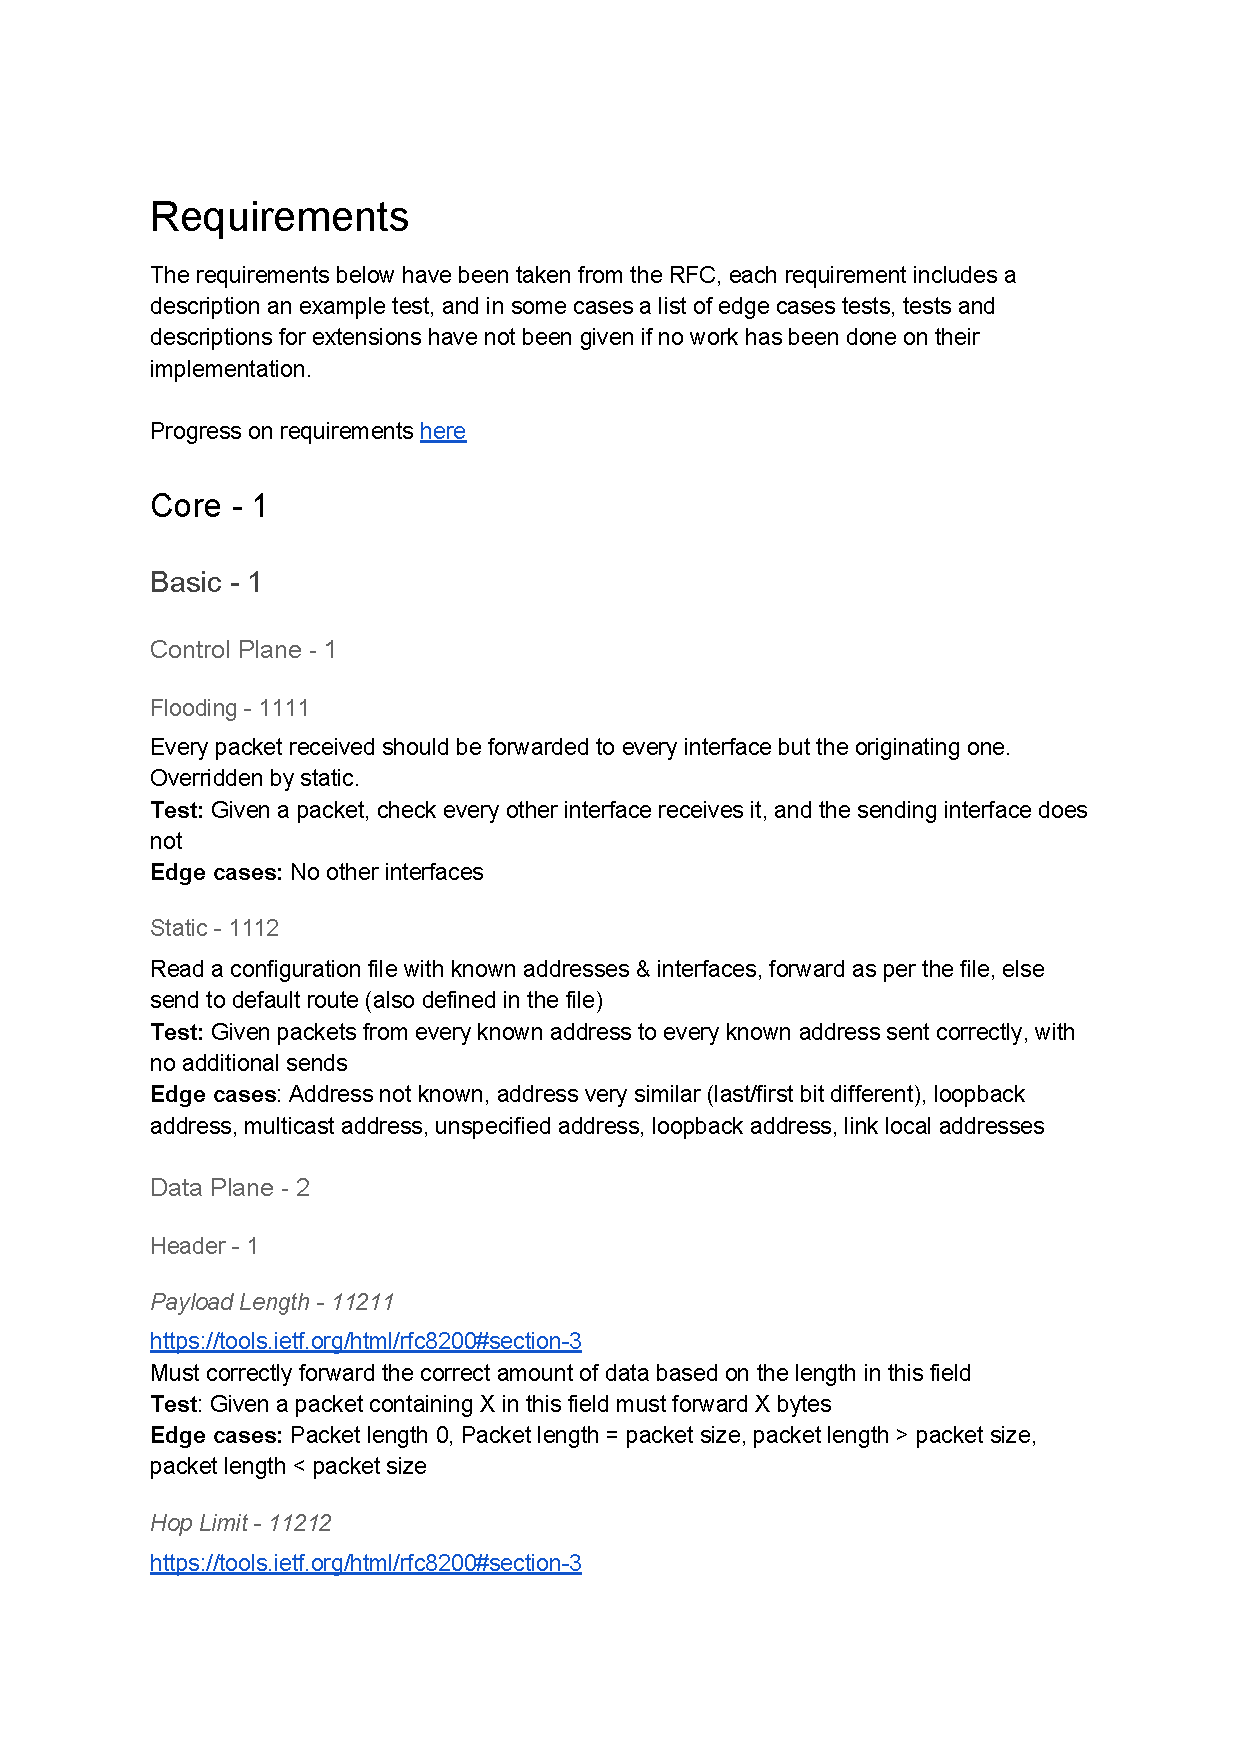
\includepdf[page=-]{requirements}


\chapter*{Project Proposal}
\label{project_proposal}
\addcontentsline{toc}{chapter}{Project Proposal}

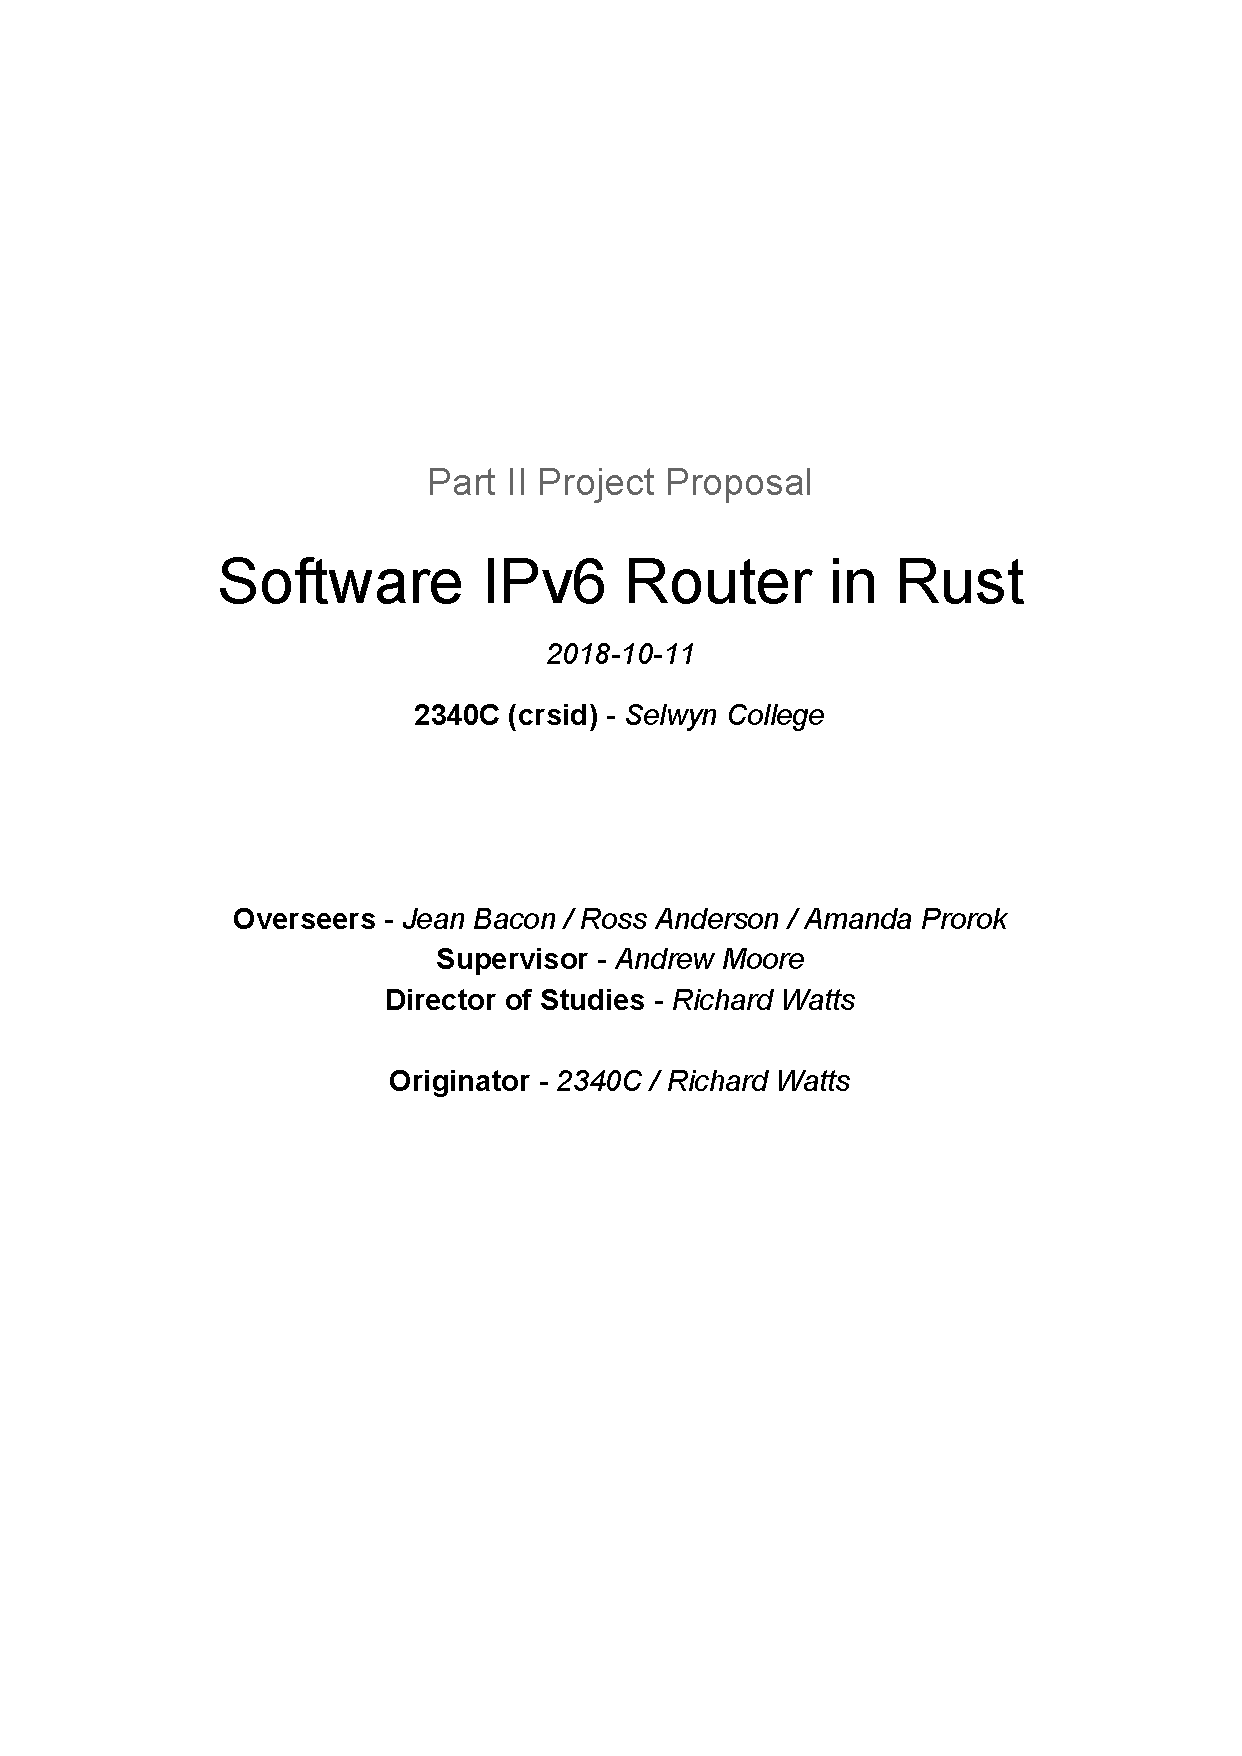
\includepdf[page=-]{proposal}

\end{document}